\documentclass[11pt]{article}

\usepackage[utf8]{inputenc}
\usepackage{graphicx}
\usepackage{geometry}
%\geometry{a4paper, margin=1in} % Adjust margins as needed
\usepackage{hyperref} % For clickable URLs
\usepackage{caption} % For customizing captions
\usepackage{booktabs} % For better tables (optional)
\usepackage{enumitem} % For customizing lists (optional)

% For math
\usepackage{amsmath}
\usepackage{amsfonts}
\usepackage{amssymb}

% For algorithms
\usepackage{algorithm}
\usepackage{algpseudocode}

% For citations
\usepackage{natbib}  

% Define some colors (optional)
%\usepackage{xcolor}
%\definecolor{darkblue}{rgb}{0,0,0.5}

% Set up title and author information
\title{Social Media Course Project \\ [1em] \Large Application of Transformer-Like Deep Neural Network Architecture For Graph Edge Prediction}
%\title{Encoder-Like Deep Neural Network Architecture For Graph Edge Prediction}
\author{Bruno Guzzo \\ 242504}
\date{Winter 2025}

% Customization for captions
\captionsetup[figure]{labelfont=bf, font=small, justification=centering, labelformat=empty, labelsep=period} % Customize as needed
\captionsetup[table]{labelfont=bf, font=small, justification=centering, labelformat=empty, labelsep=period} % Customize as needed


\begin{document}
	
	\maketitle
	
	\begin{abstract}
	This project explores the application of transformer-like Graph Neural Networks (GNNs) for edge prediction in semantic graph. The project aims to demonstrate the effectiveness of GNNs with architectural features inspired by transformer networks in capturing complex relationships and predicting potential connections within a graph dataset.
	\end{abstract}
	
	
	\section{Introduction}
	The main given guideline assignment for the present project is \textit{"Application of GNN on semantic graph generated by LLMs"}. To address such abstract assignment we chose \textit{"homemade"} approach in which we build from scratch a dataset and a neural network to solve the assignment. \\
	Our baseline idea is to build a dataset of graphs form Wikipedia article links where each node is a page title, then design a custom neural network to operate on such data type.\\
	To design such custom neural network we get inspired by the latest development in natural language processing and graph neural network. \\
	Thus, we adopt a deep neural network architecture that extend the encoder stack of the transformer \cite{vaswani2023attentionneed} with the application of graph attention network \cite{veličković2018graphattentionnetworks}.
	
	
	\section{Graph Attention}
	\label{graph_attention}
	Graph Attention Networks (GATs) are a class of neural network architectures designed to operate on graph-structured data. They leverage a self-attention mechanism \cite{vaswani2023attentionneed} to dynamically learn the importance of neighboring nodes, enabling effective feature aggregation while being independent of the underlying graph structure and allowing inductive learning.
	
	\subsubsection{Graph Attention Layer}
	The fundamental building block of a GAT \cite{veličković2018graphattentionnetworks} is the \textit{graph attentional layer}. Given a graph with $N$ nodes, each represented by a feature vector $\mathbf{h}_i \in \mathbb{R}^F$ ($i \in \{1, \dots, N\}$), the objective is to produce a new set of node features, $\mathbf{h}_i' \in \mathbb{R}^{F'}$.
	
	\subsubsection{Feature Transformation}
	Initially, each node's feature vector is linearly transformed:
	\begin{equation}
		\hat{\mathbf{h}}_i = \mathbf{W} \mathbf{h}_i,
	\end{equation}
	where $\mathbf{W} \in \mathbb{R}^{F' \times F}$ is a learnable weight matrix.
	
	\subsubsection{Attention Mechanism}
	Next, an attention mechanism is employed to compute the importance of node $j$'s features to node $i$. This is achieved through a shared attentional mechanism $a: \mathbb{R}^{F'} \times \mathbb{R}^{F'} \rightarrow \mathbb{R}$:
	\begin{equation}
		e_{ij} = a(\hat{\mathbf{h}}_i, \hat{\mathbf{h}}_j).
	\end{equation}
	In practice, $a$ is often implemented as a single-layer feed-forward neural network with parameters $\mathbf{a} \in \mathbb{R}^{2F'}$:
	\begin{equation}
		e_{ij} = \text{LeakyReLU}\left( \mathbf{a}^T [\hat{\mathbf{h}}_i || \hat{\mathbf{h}}_j] \right),
	\end{equation}
	where $||$ denotes concatenation and $\text{LeakyReLU}$ is a nonlinear activation function.
	
	\subsubsection{Masked Attention}
	To incorporate graph structure, the attention mechanism is masked. The coefficients $e_{ij}$ are only computed for nodes $j \in \mathcal{N}_i$, where $\mathcal{N}_i$ is the set of neighbors of node $i$ (including $i$ itself).
	
	\subsubsection{Normalization}
	The coefficients are then normalized using a softmax function over the neighborhood of each node:
	\begin{equation}
		\alpha_{ij} = \frac{\exp(e_{ij})}{\sum_{k \in \mathcal{N}_i} \exp(e_{ik})}.
	\end{equation}
	
	\subsubsection{Feature Aggregation}
	Finally, the new feature vector for node $i$ is calculated by aggregating the transformed features of its neighbors, weighted by the normalized attention coefficients:
	\begin{equation}
		\mathbf{h}'_i = \sigma \left( \sum_{j \in \mathcal{N}_i} \alpha_{ij} \hat{\mathbf{h}}_j \right),
	\end{equation}
	where $\sigma$ is a nonlinear activation function.
	
	\subsubsection{Multi-Head Attention}
	To stabilize the learning process and capture different aspects of node relationships, multi-head attention is utilized.  The operation of the graph attention layer is performed $K$ times in parallel, each with a separate transformation and attention parameters $\mathbf{W}^k$ and $\mathbf{a}^k$ (respectively). The output of each head is a new node feature vector, $\mathbf{h}_i^{'k}$.
	
	\subsubsection{Concatenation}
	The output from the different heads can be concatenated together:
	\begin{equation}
		\mathbf{h}'_i = \underset{k=1}{\overset{K}{\parallel}} \sigma \left( \sum_{j \in \mathcal{N}_i} \alpha_{ij}^k \mathbf{\hat{h}}_j^k \right).
	\end{equation}
	In this case, the final output feature vector will have the dimension $KF'$.
	
	\subsubsection{Averaging}
	Alternatively, for the final layers, the outputs can be averaged followed by the final activation:
	\begin{equation}
		\mathbf{h}'_i = \sigma\left(\frac{1}{K} \sum_{k=1}^K \left( \sum_{j \in \mathcal{N}_i} \alpha_{ij}^k \mathbf{\hat{h}}_j^k \right) \right).
	\end{equation}
	Here, the final output feature vector has the dimension $F'$.

	\section{Wikipedia Articles Link Dataset}
	Given the necessity of a consistent graph dataset to train our GNN we chose to build a suited dataset to address the project needs.
	Each data point of our dataset is a graph where each node is a Wikipedia article title and the edges represent links between them. The presence of an edge $(u, v)$ means that the article $u$ cite article $v$ in its body or vice-versa.
	Following this principle we obtain a non-directed graph where the edges indicate that two articles are somehow related.
	\begin{figure}[h] % h! means "here" and try hard
		\centering
		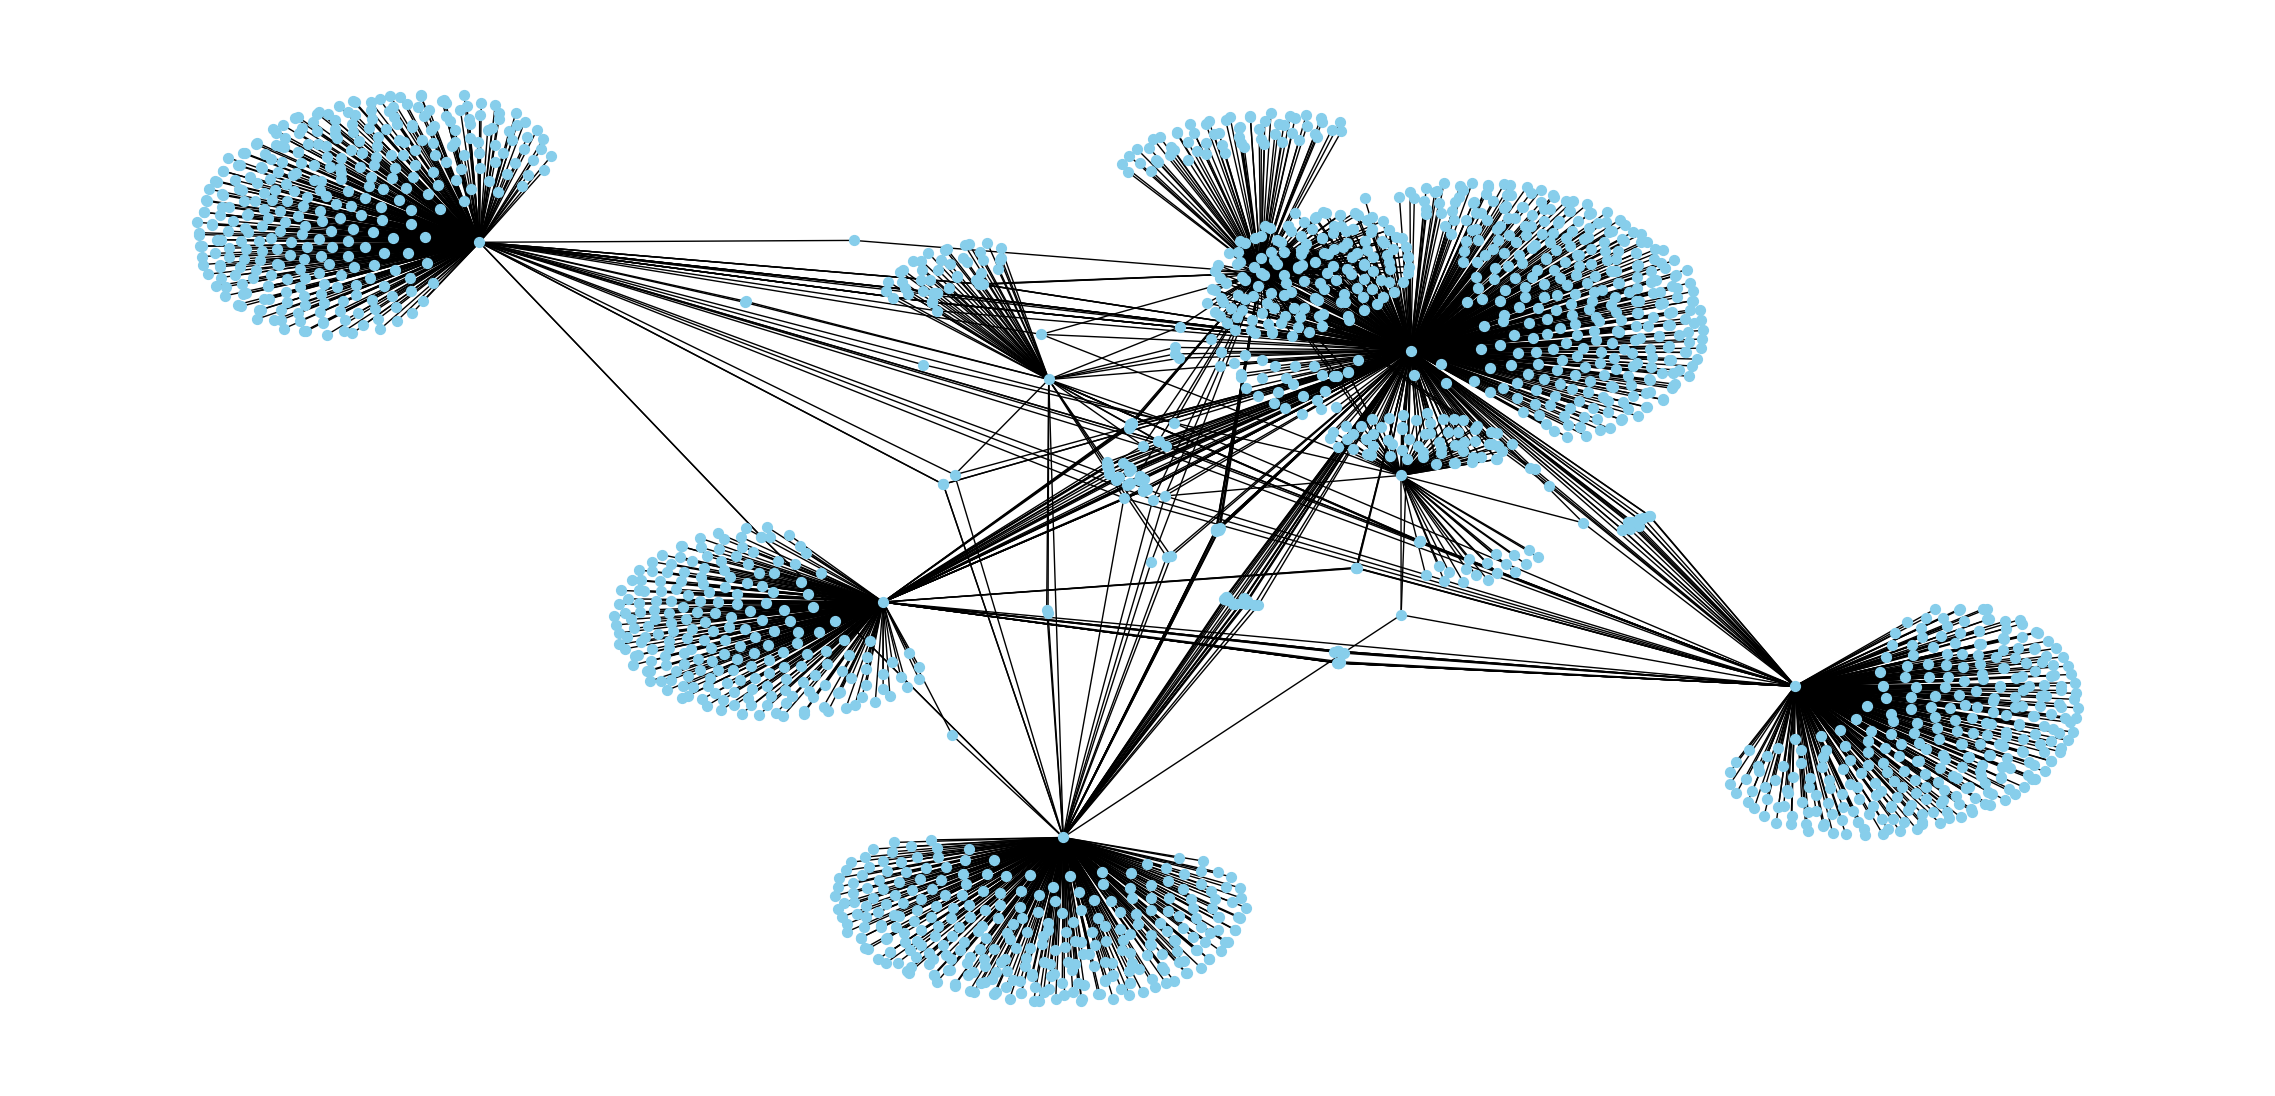
\includegraphics[width=1\textwidth]{images/wiki_link_grap_2k.png}
		\caption{Figure 1: A graph of 2000 nodes built form the root article title 'Sustainability'.}
	\end{figure}
	
	\subsection{Graph Extraction Algorithm}
	To obtain the graphs of our dataset we adopt a \textbf{breadth first strategy} to explore Wikipedia article links starting for a \textbf{root article}. This prioritize the inclusion of the immediate neighborhood of the root article.
	We adopt this methodology against a \textbf{depth first strategy} so we can have all the immediate neighbors of the root node, thus leading to a \textbf{robust representation} of the root article.
	This is particular helpful when using GNN where the network learn a node representation using the information present in it's first neighbors.\\\\
	The final graph produced by our algorithm is limited by a maximum size of \textbf{20000 nodes}. This allow us to obtain a graph that capture the deep structure of Wikipedia. \\
	Below we present a simplified \textbf{pseudo-code} of the BFS algorithm used, the final version is \textbf{recursive} and have several constraint to enforce graph consistency. 
	
	\begin{algorithm}
		\caption{Wikipedia Graph Extraction using BFS}
		\begin{algorithmic}[1]
			\Require $rootArticleTitle$, $maxNodes$
			\State $graph \gets$ new Graph
			\State $visited \gets$ new Set, initialized with $rootArticleTitle$
			\State $queue \gets$ new Queue, enqueue $rootArticleTitle$
			\State $graph$.addNode($rootArticleTitle$)
			\While {$queue$ is not empty and $|graph.nodes| < maxNodes$}
			\State $pageTitle \gets queue$.dequeue()
			\State $page \gets$ getWikipediaPage($pageTitle$) \Comment{Handles Page/Disambiguation Errors}
			\If {$page$ is not valid}
			\State \textbf{continue} \Comment{Skip to the next page in queue}
			\EndIf
			\For {$linkTitle$ in $page.links$}
			\If {$|graph.nodes| \geq maxNodes$}
			\State \textbf{break} \Comment{Exit loop}
			\EndIf
			\If {$linkTitle \in visited$}
			\State $graph$.addEdge($pageTitle$, $linkTitle$)
			\Else
			\State $visited$.add($linkTitle$)
			\State $queue$.enqueue($linkTitle$)
			\State $graph$.addNode($linkTitle$)
			\State $graph$.addEdge($pageTitle$, $linkTitle$)
			\EndIf
			\EndFor
			\EndWhile
			\If {not isConnected($graph$)}
			\State \textbf{Error:} Graph is not connected
			\EndIf
			\State \textbf{return} $graph$
		\end{algorithmic}
		\label{alg_1}
	\end{algorithm}
	
	\subsection{Node Embedding}
	To efficiently use our dataset with GNN it is needed to \textbf{embed each node} in way that it can be processed in a numerical way. To do so, we relay on state-of-the-art sentence embedding model to transform node labels in numeral representation.
	We chose to use a freely and open-source available \textbf{sentence-transformers} model: \textbf{\href{https://huggingface.co/sentence-transformers/all-MiniLM-L6-v2}{all-MiniLM-L6-v2}} \cite{reimers-2019-sentence-bert}. \\\\
	It maps sentences and paragraphs to a \textbf{384 dimensional dense vector space} and can be used for tasks like \textbf{clustering} or \textbf{semantic search}.
	\textbf{all-MiniLM-L6-v2} is derived from the MiniLM \cite{wang2020minilmdeepselfattentiondistillation} architecture and it leverages a distilled version of the \textbf{BERT} (Bidirectional Encoder Representations from Transformers) \cite{devlin2019bertpretrainingdeepbidirectional} model.\\
	The description of this model is outside the scope of this project and it is already been exposed in our previous natural language processing project.,
	
	\subsection{Final Dataset}
	The final dataset has been generated by executing the \textbf{algorithm \ref{alg_1}} on a list of Wikipedia article titles and saving the graph information (nodes and edges) in JSON files.
	We used a list of Wikipedia article titles related to \textbf{sustainability and development} (around $300$), but we have also included the \textbf{top 50 most visited} article in 2024.
	This would ensure that the final GNN model will preserve a small but broad \textbf{generalization capability}.\\\\
	However, to ensure fast data loading, we have also created a \textbf{tensor} file version of the dataset which include node embedding and labels as well.
	Thus, the final dataset is composed of \textbf{389 graphs} with \textbf{20000 nodes each}, this amount to roughly \textbf{7 million of nodes}. It worth it to note that, of course, some graphs could share common node labels.\\
	
	
	\section{Graph Neural Network Architecture}
	Before to get to the final network architecture it is important to remark decisions and ideas that lead us to develop such architecture. 
	\begin{itemize}
		\item{\textbf{Problem complexity}}: The link prediction task is not easy, especially when dealing with thousands of nodes and edges. It is needed to capture relation between distant nodes. So, the propagation of the information form nodes to nodes is crucial to ensure optimal result. For this reason, we could hypnotize the need for a \textbf{deep neural network} to address the long information transfer needed. 
		
		\item{\textbf{Dealing with graphs}}: Each data point of our dataset ia a huge graph, so it is needed to use state-of-the-art graph neural network methodology to deal with such objects. We chose to adopt the aforementioned \textbf{graph attention} \cite{veličković2018graphattentionnetworks} \ref{graph_attention} since it has shown better results than convolutional graph neural network \cite{kipf2017semisupervisedclassificationgraphconvolutional}. 
		
		\item{\textbf{Dealing with words}}: Despite he graphic nature of the problem we are fundamentally trying to learn relation from words and small phrases. This is a common problem of \textbf{NLP} (Natural Language Processing). So, it is natural to look to the solutions applied in such filed to take inspiration from. This intuition lead us to chose a sub-layer structure similar to the one used in the well-known \textbf{transformer architecture} \cite{vaswani2023attentionneed}.   
	\end{itemize}
	
	\subsection{Network Architecture In Detail}
	\begin{figure}[h] % h! means "here" and try hard
		\centering
		\label{figure_2}
		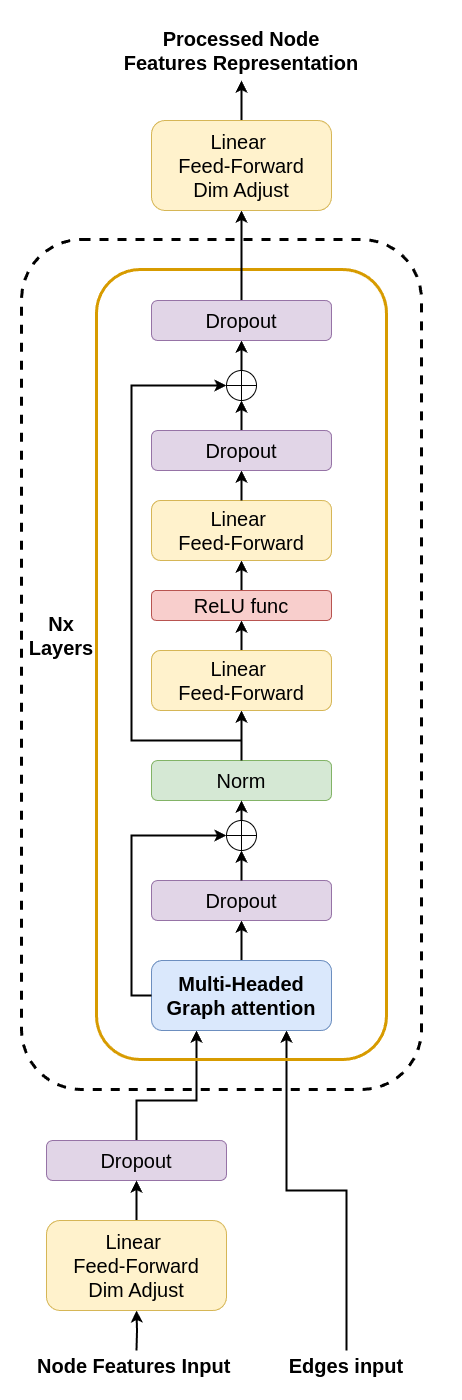
\includegraphics[height=0.8\textwidth]{images/custom_gnn_diagram.png}
		\caption{Figure 2: Graphical representation of the our final \textbf{graph neural network}.}
	\end{figure}
	
	
	
	\subsection{Chosen Architecture Parameters}
	
	\section{Network Training}
	
	\section{Link Prediction Task Results}
	
	\section{Methodology}
	
	Describe the methods you used to conduct your project. This might include data collection methods (e.g., surveys, interviews, social media data analysis), data analysis techniques, tools used, and any specific procedures you followed. Be clear and detailed enough so that someone else could replicate your work.
	
	\section{Results/Findings}
	
	Present your findings in a clear and organized manner.  Use figures, tables, and other visual aids to illustrate your results effectively.  Make sure your visuals are properly labeled and captioned.
	
	%\begin{figure}[h!] % h! means "here" and try hard
	%	\centering
	%	\includegraphics[width=0.8\textwidth]{placeholder_image.jpg} % Replace with your image file
	%	\caption{Figure 1: Description of your figure.}
	%\end{figure}
	
	\begin{table}[h!]
		\centering
		\begin{tabular}{lcc}
			\toprule
			Variable & Value 1 & Value 2 \\
			\midrule
			Result 1 & 10 & 20 \\
			Result 2 & 30 & 40 \\
			\bottomrule
		\end{tabular}
		\caption{Table 1: Description of your table.}
	\end{table}
	
	\section{Discussion}
	
	Interpret your results and discuss their implications.  What do your findings mean?  How do they relate to your research questions or objectives?  Discuss any limitations of your study and suggest areas for future research.
	
	\section{Conclusion}
	
	Summarize your key findings and conclusions.  Restate the significance of your project and its contributions to the field.
	
	\bibliographystyle{plainnat}
	\bibliography{papers.bib}
	
	
\end{document}